\chapter{Introduction}
We present an implementation of the future programming model for distributed memory,
using MPI-2's one-sided communication.  The interface is implemented as a runtime 
library that allows the user to  expose parallelism, by issuing callable functor object 
asynchronously.  The future object is used a simple communication channel, where the worker process 
will send through it the return value of the functor object. 
A future object is also used for synchronization. Such an object can be accessed at any time during execution,
but the process accessing it will block until the worker process finishes the execution of functor object, and
transmits the result to the future object.

\paragraph{}
Traditionally implemented using threads over shared memory environments.  
In this work we show that the C++11 standard future interface~\cite{CPP:Threads} can be implemented meaningfully 
for distributed memory machines.  We have chosen to build our system using the MPI-2 one-sided
communication library, so that we can explore and evaluate it's potential to provide a completely asynchronous
communication scheme.  Another reason for using an MPI library is that it is the most commonly message passing
library available on distributed and shared memory machines alike.  
The contributions of this work can sum up to:
\\
\begin{itemize}
	\item Implementation of the C++11 futures interface for distributed machines, as a runtime system.
	\item Performance Evaluation of the our implementation. 
	\item Evaluation of the MPI-2 one-sided communication interface, for implementing an advanced runtime system.
	\item Exploration of the potential of implementing a runtime on distributed memory using shared memory scheduling techniques.
\end{itemize}

\paragraph{}
Our evaluation shows that the interface implementation is possible, but, performance-wise,  our implementation 
is only able to offer some speedup only when we use coarse grain tasks, due to the high cost of issuing functions 
asynchronously and/or inefficient synchronization schemes. Moreover, MPI-2 one-sided communication interface is 
not as versatile as we would like, and forces some limitations, especially on fine grain synchronization.  

\paragraph{}
The rest of this report is organized as follows:  In the rest of the introduction, we present the current state
and trends in parallel computing.  We briefly introduce the concept of asynchronous execution models and present
the futures programming model.  At the end of the introduction, we describe MPI's one-sided communication interface.
In chapter \ref{chap:related} we discuss other projects related with our work, and present their approach to
asynchronous communication.  In chapter \ref{chap:implementation} we present in details our system's design and 
implementation.  In chapter \ref{chap:evaluation} we assess our efforts to build the C++11 interface using 
MPI's one-sided communication and use some microbenchmarks and real applications to evaluate the performance
of our runtime system.  Finally, in chapter \ref{chap:conclusion} we give our concluding remarks, regarding our
work and our assessment of the one-sided communication interface of MPI, along with our suggestions for its 
improvement.    


\section{Parallel Computing}
\paragraph{}
	High performance computing is today strongly related with parallel programming.  On one end, computer
architectures have been developing parallel machines or netword configurations for clusters of machines
in order to increase performance, and on the other, researchers have been trying to develop programming
models that will allow programmers to develop or port efficiently their applications to these emerging 
technologies.  When developing parallel applications the two most dominant and widely used programming 
models are threads and message passing.  

\paragraph{}
Threads model is commonly used on shared memory machines, where 
the communication scheme would have one thread writing to a memory location
and another thread reading the data from that location.  This model does not require data to be
transfered among threads but can lead to race conditions when two threads try to access the same
data at the same time or, if a thread does not respect RAW and WAR dependencies. 
In order to ensure correct program execution,
the user must synchronize memory access by the threads using mutexes, semaphores, locks, barriers etc.
Correct synchronization has proven to be a daunting and error-prone task for programmers, and often 
synchronization bugs in application can be the cause for  
erroneous results, or even worse, deadlocks.  Pthreads and OpenMP~\cite{Dagum:1998:OIA:615255.615542}
 are two commonly used libraries
that are used to program threads on shared memory machines.  With Pthreads the user can create and
launch and threads, where each thread will have a specific work to do.  The library also offers 
a variaty of synchronization primitives such as locks, barriers, mutexes etc.  OpenMP offers
a higher abstraction level interface, where the programmer uses special \#pragmas to annotate
code sections that should be executed in parallel.  These pragmas can denote loops that should 
be run in parallel or even organize parallel work into tasks~\cite{Ayguade:2009:DOT:1512157.1512430},
while the library takes care of creating and launching threads.  However, the user is again responsible
for synchronizing data accesses.

\paragraph{}
In contrast with the threads model,  applications using the message passing model, use messages to share data
between different processes and also for synchronization.  The usual scheme requires a matching pair
of send and receive operations where both application will have to eventually block at some point until
the message has been received. Although the message passing model is considered more difficult to program 
than programming with threads on shared memory, it is easier to reason about data locality, thus can 
potentially achieve very good performance.  Moreover, message passing libraries are usually the only 
available option on large scale distributed machines, where different physical nodes do not share 
a global address space.  A drawback of most message passing implementations is that two-sided 
communication is required when exchanging messages.  This means that both sender and receiver must
take active part in the communication, which usually means that both need to block at some point,
until the message is sent/received.  

\paragraph{}
An alternative from the usual message passing two-sided communication model, 
is the one-sided communication model, where one process can remotely write
or read from the address space of another process, while the latter is not required 
to take active part in the transaction.  ARMCI~\cite{Nieplocha99armci:a} 
LAPI~\cite{Shah:1998:PEL:876880.879642} and MPI-2 provide library implementations of such 
one-sided communication interface. OpenSHMEM~\cite{Chapman:2010:IOS:2020373.2020375} is 
an effort to standardize the SHMEM. An attractive property of this model, is that communication can happen 
asynchronously, which also means however that the programmer needs to explicitly synchronize
processes as in the shared memory model, using barriers and fences.  

\paragraph{}
The emerge of the one-sided communication model has made it possible to develop libraries and languages
that follow the PGAS \emph(Partitioned Global Address Space) programming model.  In this model,
a virtual global address space to the programmer, when in fact, this address space is 
distributed among the different nodes or a logical partition dedicated to a single thread.  
This model tries again to exploit the benefits of the message passing's SIMD model while providing
an easy way to address data as in the shared memory models.  UPC, Chapel and Fortress are languages
that use the PGAS model and are built ontop of a one-sided communication library.  
Global Arrays~\cite{Nieplocha:2006:AAP:1125980.1125985} is also
an API that follows the PGAS model and is built ontop on ARMCI~\cite{Nieplocha99armci:a}. 

\paragraph{}
Because all of the previous models are either considered difficult to program or error prone, a lot of higher 
level programming models have been suggested in the literature, that are implemented on top of one of the 
previous, lower level, ones.  The concept of organizing parallel work in functions that can be run
concurrently has lead to the development of many task-based programming models
~\cite{Ayguade:2009:DOT:1512157.1512430, Blumofe95cilk:an} in the shared memory
environment and to similar models in distributed memory like Remote Procedure Calls (RPC)
~\cite{Saunders:2003:AAP:966049.781534,Beckman96tulip:a,Vadhiyar03gradsolve-}
or Remote Service Request (RSR) ~\cite{Foster96thenexus}.  Although this higher level
abstraction makes it easier to organize parallel code in tasks, it is still up to the 
programmer to explicitly synchronize data accesses between tasks, using barriers, etc.
To address and simplify the synchronization problems, a lot of systems have been suggested
in the literatture, that provide implicit synchronization.  In the scope of task based parallel
models, these systems usually require some sort of task memory footprint description from the 
programmer~\cite{Tzenakis:2012:BBD:2370036.2145864, Perez:2010:HTD:1810085.1810122}
and/or have the compiler statically infer dependendencies among tasks 
~\cite{Jenista:2011:OSO:1941553.1941563, Zakkak:2012:IDI:2370816.2370892}.
This scheme usually allows the programmer to describe the data-flow relations between different
parallel tasks, and an underlying runtime systems will explicitly synchronise them.  The drawback
here is that there is usually an additional overhead from the runtime system and/or the automatic
(dynamic or static) analysis used to automatically synchronise the code, is often conservative
in order to maintain correctness, which harms performance.

\section{Futures and Promises}
\label{sect:futures-promises}

\paragraph{}
Experience with parallel programming has shown that common synchronization techniques like
barriers do not scale well on massively parallelization machines ~\cite{4100352}, with thousands of workers.
We would like to use finer grain synchronization, but reasoning about the exact point an operation will complete
is virtually impossible in a parallel environment.  An alternative is to use asynchronous programming models, which
allows the programmer to write programs where a thread or process can be oblivious to what actions the other threads/
processes are doing, while he can still retrieve the results of concurrent work and produce the correct result.

\paragraph{}
The futures (or promises) model is such an asynchronous programming model.  A future is a special variable which may 
or may not have a value at the time that it is referenced in program.  Usually a future is coupled with a promise.  
A promise is a special construct that is associated with a future and can be used by another thread or process to 
set the value of the future variable.  Usually, the future is used only to read the variable value, while the 
promise is used to write to the same variable, thus defining a data-flow relation between different threads/processes.
The promise construct is often hidden from the programmer, where instead he will have to declare a callable object
(function, functor, etc) and the library will offer a mechanism to use this callable object to set the future through 
the promise, after executing the user's callable object.  Such is the use of the \emph{async} function in the C++11 
standard, where the user can issue a function or functor object and retrieve a future object using the \emph{async} call.
The async will be run by a thread, and the return value of the function or functor will be used to set the future object 
associated with the \emph{async} call.   

\begin{figure}[!ht]
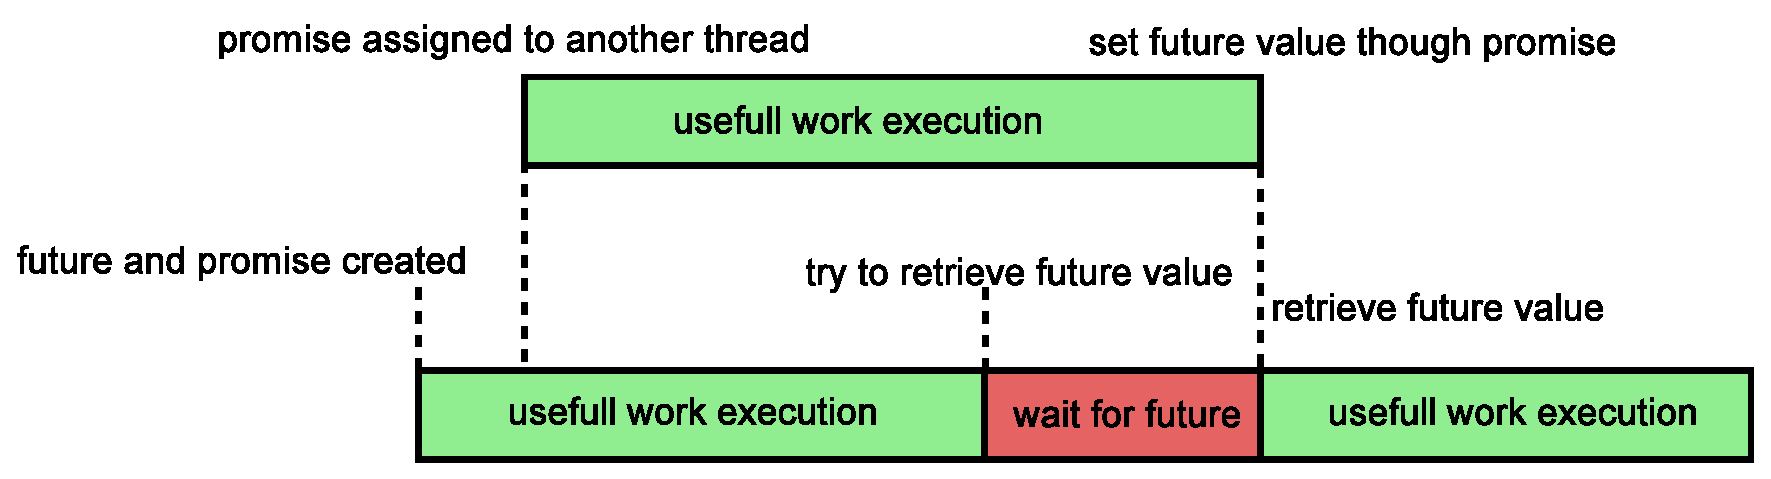
\includegraphics[width=\columnwidth]{figures/futures_blocking}
\caption{
The futures execution model of the blocking schematics.}
\label{fig:futures_blocking}
\end{figure}

An important design decision for any futures implementation, is what happens when a future is referenced, while its value
is not yet available.  A common choice, is to have the caller block until it the future value is resolved or implicitly
try to resolve the future at the reference time (as with lazy evaluation schemes).  Figure \ref{fig:futures_blocking} 
shows the execution model of the blocking scheme.  The green color is the time a thread spends doing useful computation, 
while the red color is the idle time a thread spends on waiting for the result of the future. This is the scheme used by C++11, 
an alternative is the Scala future implementation~\cite{Scala:Futures}, where the user can set a callable object to be
called when the future will be set, or if the future throws an exception (failure), using the callback mechanism.  This scheme
has the benefit that there will be no blocking at any point of the code, allowing true asynchronous execution.  The C++11
standard, as most blocking future implementations, offer the option to ask whether a future is ready before referencing its 
value, in order to avoid any blocking if possible. 

\begin{figure}[!ht]
\begin{lstlisting}
int	fibonacci(int n) {
	if(n == 0) return 0;
	if(n == 1) return 1;
	return fibonacci(n-1) + fibonacci(n-2);
}
\end{lstlisting}
\caption{A sequential fibonacci implementation}
\label{lst:fib_seq}
\end{figure}

\begin{figure}[!ht]
\begin{lstlisting}
int	fibonacci(int n) {
	if(n == 0) return 0;
	if(n == 1) return 1;
	future<int> fib1 = async(fibonacci, n-1);
	future<int> fib2 = async(fibonacci, n-2);
	return fib1.get() + fib2.get();
}
\end{lstlisting}
\caption{A fibonacci implementation using the C++11 futures interface}
\label{lst:fib_futures}
\end{figure}

\paragraph{}
Other than the asynchronous execution model they use, we believe that another attractive property of the futures model 
is that they can be used to compose easy to use interfaces, with higher level abstractions that the programmer can use 
in order to develop parallel applications.  As a motivation to the reader, we present in figure \ref{lst:fib_futures} a
Fibonacci function implementation, using the C++11 standard threads library~\cite{CPP:Threads} future interface.  Figure
\ref{lst:fib_seq} also shows the sequential equivalent.  The parallel version simply requires the recursive calls 
to be issued using the \emph{async} function, and the use of the get method on the future objects in order to retrieve
the return values, of the recursive calls.  Note, that the call to the get method here is blocking.  


\section{MPI one-sided communication}
\label{sect:mpi-one-sided}
\paragraph{}
One of the most controversial features of MPI-2 is it's one-sided communication.  Although PGAS programming
models and languages have become widely accepted for developing code in large scale machines, programmers
consider the MPI one-sided communication interface to be generally difficult to understand and use.  In this
section we try to familiarize the reader with the main concepts of the interface.  

\paragraph{}
In order to perform remote access operations on some data, this data, residing on one process, needs to be exposed to 
the other processes, through an MPI\_Window object.  Thus, all processes need to create an MPI\_Window that will expose
part of their local address space to all other processes.  MPI\_Windows are created using the MPI\_Win\_create function.
This functions requires a pointer to a local address space and the size of the data to be shared, through the window.
This is a collective operation over a group of MPI processes.  Each process can expose different size of data (or none)
to the window. Note that only the processes in the group will be able
to perform a remote operation on the created MPI\_Window.

\paragraph{}
The two main operations that can be performed are MPI\_Put and MPI\_Get, which allow a process to remotely write and
read some data respectively.  Both operations are applied on an MPI\_Window and the rank of the process, whose address
space  we want to remotely write to or read from.  In addition, a buffer has to be supplied to each function, that
either points to the data that needs to be written to the remote address or to the local memory that the remote data
will be stored to.  Along with the buffers, an MPI\_Datatype and buffer size must be supplied.  Another operation 
available is the MPI\_Accumulate, that can be used to apply some action on the data that is remotely read and the local
data on the process.  An operation must also be supplied to this function.    

\paragraph{}
In contrast to the two-sided communication interface, in the one-sided interface, get and put operation need not 
be paired and non-blocking, thus synchronizing processes that perform these remote operations must be explicitly
done by the programmer.  Synchronization in the MPI one-sided communication interface is achieved using "epochs",
that define the start and end of an operation.  All one-sided operations must happen in one "epoch".  MPI provides
two different ways to define "epochs", called \emph{active target} and \emph{passive target}.

\paragraph{}
In the \emph{active target} mode both processes are required to take part in the synchronization.  The programmer 
need to declare the beginning and end of an "epoch" in the origin process, by explicitly calling MPI\_Win\_start/complete.
On the target process, MPI\_Win\_post/wait must be used to declare the beginning and end of the "epoch".  MPI\_Win\_start needs
to be paired with an MPI\_Win\_post and MPI\_Win\_complete must be paired with an MPI\_Win\_wait.  Moreover, an "epoch" can be 
defined by using a pair of MPI\_Win\_fence calls to declare the start and end of the "epoch".  This function is used for 
collectively synchronizing remote operations.  All these functions require an MPI\_Window to be provided as an argument. 

\paragraph{}
The \emph{passive target} mode requires only the origin process to define the start and end of an "epoch", by using 
MPI\_Win\_lock/unlock respectively.  Again, the window on which the operation is performed is required to be passed as
an argument along with the rank of the target process.  An MPI\_Win\_lock/unlock can be either shared or exclusive.
A shared lock allows or concurrent operations to take place in the same "epoch", while the exclusive will force them
to happen in different "epochs".  However, note that concurrent conflicting accesses to the same MPI\_Window can be 
erroneous, and MPI locks are not to be confused with mutual exclusion schemes.
 

